\section{Evidence and Reproduction}
\label{sec:evidence}
\subsection{What the original paper establishes}
\label{sec:csa-paper-evidence}
The paper evaluates reconstruction on ORL and CMU PIE and recognition on ORL,
CMU PIE, FERET, and MNIST. For reconstruction, one image per identity is used;
the compression ratio counts both shared projection matrices and per-image
coefficients. The paper's Figure~5 reports lower reconstruction RMSE for CSA at comparable
storage budgets. Its Figure~4 shows near-stable projections by approximately three
iterations in the illustrated ORL run, an empirical observation rather than a
universal bound. Recognition uses 1-NN with optional LDA, including ORL's
two-gallery/eight-probe split and FERET's disjoint training/test identities.
Table~\ref{tab:recognition} reproduces selected paper results: for Gabor ORL,
direct CSA reaches 94.40\% with 390 coefficients versus PCA's 86.60\% with 76.
These support the reported configurations; they do not isolate representation
quality at equal output dimension. The authors report best parameter settings,
with repeated-split aggregation unspecified \citep[Sec.~IV]{xu2008csa}.

\subsection{Our implementation and scope}
We independently implemented CSA, PCA, Fisher LDA, and evaluation code using
NumPy/SciPy for numerical operations and Pillow/OpenCV for image processing;
YuNet detection assets are reused. We reproduced ORL, MNIST, and original
grayscale FERET experiments; CMU PIE was unavailable and omitted with instructor
permission. Code, run instructions, provenance, and recorded results are at
\url{https://github.com/gwdsd1/COMP3314GP}.

ORL uses ten splits with two gallery and eight probe images per identity;
MNIST uses three splits with 30 or 40 training images per digit; FERET uses one
fixed identity partition for each training size. Methods share input arrays,
splits, and distance within each comparison: Euclidean for current ORL and
cosine for MNIST/FERET. Recognition PCA is centered and CSA uncentered, so this
does not isolate the projection constraint under identical centering.
ORL preprocessing retains earlier probe-informed exploration, including the
Gabor context extension. These scores are not fresh blind-test estimates.
Appendix~\ref{app:protocol} details input conventions and deviations from the paper.

\subsection{Results and controlled comparisons}
\begin{table}[!ht]
\centering
\small
\setlength{\tabcolsep}{4pt}
\caption{Top-1 accuracy (\%). Paper columns are from \citet{xu2008csa},
Tables I, II, and IV; ours are recorded group experiments, not new runs for this
report. ORL/MNIST show mean $\pm$ sample SD over ten/three splits; FERET uses
one partition per training size. Dimensions follow each paper configuration.}
\label{tab:recognition}
\begin{tabular}{@{}lrrrr@{}}
\toprule
&\multicolumn{2}{c}{PCA}&\multicolumn{2}{c}{CSA}\\
\cmidrule(lr){2-3}\cmidrule(l){4-5}
Setting&Paper&Ours&Paper&Ours\\
\midrule
ORL gray + LDA&82.20&$77.22\pm2.35$&84.10&$81.72\pm2.06$\\
ORL Gabor, direct NN&86.60&$86.91\pm1.60$&94.40&$89.66\pm1.92$\\
ORL Gabor + LDA&87.20&$88.41\pm1.96$&90.90&$87.53\pm2.91$\\
MNIST, 30 train/class&88.50&$87.52\pm0.40$&92.80&$90.34\pm0.15$\\
MNIST, 40 train/class&90.50&$88.58\pm0.37$&92.40&$91.04\pm0.25$\\
FERET, 50 train identities&84.60&89.08&88.20&88.73\\
FERET, 100 train identities&90.60&90.87&92.20&94.25\\
FERET, 200 train identities&93.40&93.87&95.20&95.38\\
\bottomrule
\end{tabular}
\end{table}
\FloatBarrier

CSA exceeds our PCA baseline in six of eight configurations. MNIST preserves
the paper's CSA-over-PCA ordering; FERET CSA matches or exceeds its reported
values, but loses to our PCA at 50 training identities. All three ORL CSA means
remain below the paper. Our ORL reconstruction and projection-stabilization
records recover the qualitative trends (Appendix~\ref{app:reconstruction}),
rather than exact author-identical curves.

The Gabor LDA row compares CSA $24\to23$ with PCA $33\to25$.
Matching both at $24\to23$ yields 87.53\% versus 85.72\% under Euclidean distance,
a CSA advantage of 1.81 percentage points. Applying centered cosine to the same
fitted models instead gives 88.75\% versus 90.59\%, reversing the ordering.
Figure~\ref{fig:metric} shows that recognition gains depend on the metric, even
with fixed representations.
In a separate 20-split centered-cosine control at Gabor $\sigma=\pi$, extending filtering beyond
the crop raises CSA from 81.25\% to 87.08\%, while matched context PCA reaches
91.08\%. Better preprocessing therefore need not establish a CSA advantage.

\begin{figure}[!ht]
\centering
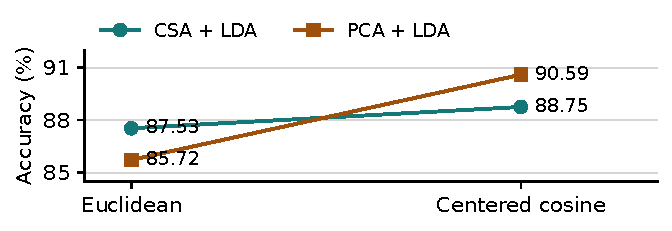
\includegraphics[width=0.78\linewidth]{figures/metric_comparison.pdf}
\caption{Our matched-dimension ORL Gabor results: ten-split means for
CSA and PCA, both $24\to23$. Only the distance rule changes between columns;
the fitted models and splits are fixed. Source: group records listed in
Appendix~\ref{app:controls}.}
\label{fig:metric}
\end{figure}
\FloatBarrier
